\section{Cross Sections}

To predict the cross section properties, iStructure implements the \textit{section properties} Open Source library \cite{secprop}. With the material of the structural members chosen, the next step should be to establish a database of structural profiles. By default, the software use square sections for columns, I section for beams and C section for joists. Other kinds of sections are also supported, including user custom sections. For example, for a joist, Cee section, you simply specify the dimensions, as shown on Listing 1.

\begin{lstlisting}[language=Python, caption=Cee section definition]
from sectionproperties.pre.sections import CeeSection
cee = CeeSection(d=120, b=60, l=15, t=4, r_out=5.4, n_r=8)
cee.plot_geometry()
\end{lstlisting}

Cee cross section scheme can be appreciated on figure \ref{cScheme}.

\begin{figure}[h!]
\centering
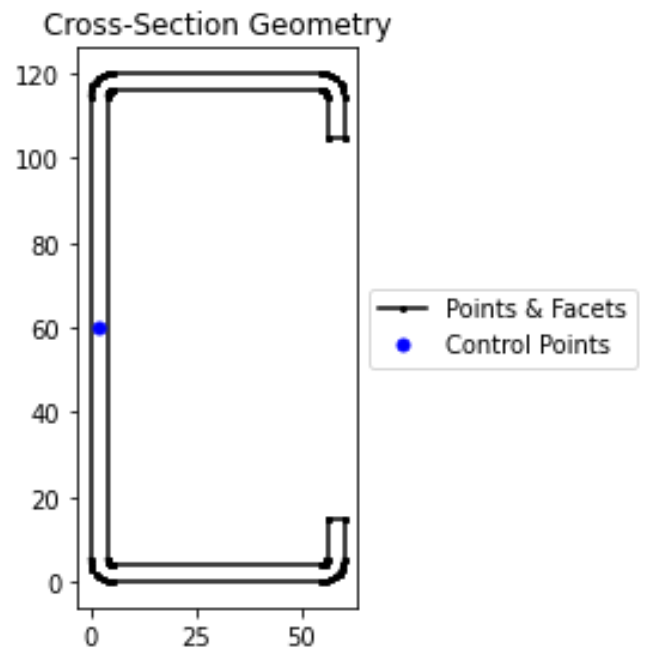
\includegraphics[width=0.8\textwidth]{Images/sections/cee.PNG}
\caption{Cee section.}
\label{cScheme}
\end{figure}

Geometric, plastic and warping analysis is developed by a Finite Element Method simulation of the cross section. We start by applying the discretization of the domain.

\begin{lstlisting}[language=Python, caption=Cee section definition]
from iStructure.CrossSection.MechProp import CrossSection
from iStructure.CrossSection.GenericMaterials import steel
mesh = cee.create_mesh(mesh_sizes=[3.0])
ceeSection = CrossSection(cee, mesh, [steel])
ceeSection.display_mesh_info()
\end{lstlisting}

With this configuration, a regular tetrahedral mesh, with elements of $3[mm]$ has been developed and can be appreciated next.

\begin{figure}[h!]
\centering
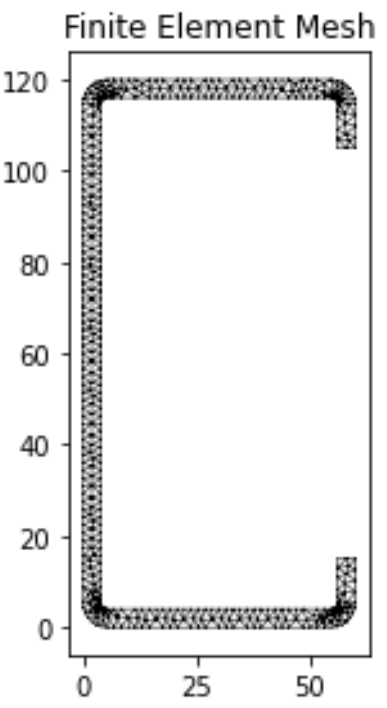
\includegraphics[width=0.45\textwidth]{Images/sections/ceeMesh.PNG}
\caption{Cee section mesh.}
\label{cMesh}
\end{figure}

\subsection{Cross section properties and FEM formulation}

\vspace{0.5cm}

\subsubsection{Problem statement}

The geometrical and wrap properties are calculated by the Finite Element Method. For the 2D linear elasticity problem, the unknown displacement field $u$, taking values in $\Omega \subset \mathbb{R} ^2$, is the solution of the boundary value problem, given by:

\begin{equation}
- \nabla \cdot \sigma (u) = b \quad \quad \quad \quad  \text{in } \Omega
\end{equation}

\begin{equation}
\sigma (u) \cdot n = t \quad \quad \quad \quad \quad  \text{on } \Gamma _N
\end{equation}

\begin{equation}
u = 0 \quad \quad \quad \quad \quad \quad \quad \text{on } \Gamma _D
\end{equation}

Where $\Gamma _N$ and $\Gamma _D$ denote the Neumann and Dirichlet boundaries with $\partial \Omega = \Gamma _N \cup \Gamma _D$  and $\Gamma _N \cap \Gamma _D = \emptyset$. The Dirichlet boundary condition in (3) is assumed to be homogeneous. The weak form of the problem reads: Find $u \in V$ sucha that

\begin{equation}
\forall v \in V \quad \quad \quad a (u,v) = l(v)
\end{equation}

where V is the standard test space for the elasticity problem such that $V = {v | v }$, and 

\begin{equation}
	a (u,v) = \int _\Omega \epsilon (u ) ^T D \epsilon (v) d \Omega = \int _\Omega \sigma (u)^T D ^{-1} \sigma (v) d\Omega
\end{equation}

\begin{equation}
l (v) := \int _\Omega b^T v d\Omega + \int _{\Gamma _N} t^T v d \Gamma
\end{equation}

where $D$ is the elasticity matrix of the constitutive relation $\sigma = D \epsilon$, $\sigma$ and $\epsilon$ denote the stress and strain operators.

\subsubsection{Finite element formulation}

Let $u ^h$ be a finite element approximation to $u$. The solution lies in a functional space $V ^h \subset V$ associated with a mesh of isoparametric finite elements of characteristic size h, which is defined by equation (3). 

Using a variational formulation of the problem (1-3) and a finite element approximation $u^h = N u^{e}$, where $N$ denotes the shape functions of order $p$, we obtain a system of linear equations to solve the displacements at nodes $u^e$:

\begin{equation}
K U = f
\end{equation}

where $K$ is the stiffness matrix, $U$ is the vector of nodal displacements and $f$ is the load vector.


\subsection{NN mesh validation}

For mesh validation error, an internal neural network algorithm has been implemented.